\section{Kubanisches Reisgericht}
% Linke Seite: Rezept
Zutaten (4 Personen):
\begin{itemize}
    \item 3 Bananen
    \item 1 Zwiebel
    \item 1 grüne Paprika
    \item 1 Dose Tomaten
    \item 1-2 Knoblauchzehen
    \item 1 Dose Kidneybohnen
    \item Salz und Pfeffer
    \item 250g Reis
\end{itemize}

\noindent Zubereitung:

\noindent Zwiebeln, Knoblauch und Paprika klein schneiden und etwas Öl
anschwitzen. Tomaten,Reis und etwa 450 ml Wasser dazugeben und mit Salz und
Pfeffer würzen. Umrühren und aufkochen lassen und bei schwacher Hitze etwa 25
Minuten köcheln lassen, bis der Reis gar ist. Bei Bedarf mit Paprika-Pulver
oder Mexiko-Pulver würzen (ist aber nicht nötig).

\noindent Bananen halbieren und in einer Pfanne bei mittlerer Hitze anbraten,
bis sie leicht karamellisiert sind. Zum Reis servieren.

% Recht Seite: Bild
\newpage
\mbox{}
\vfill
\begin{center}
    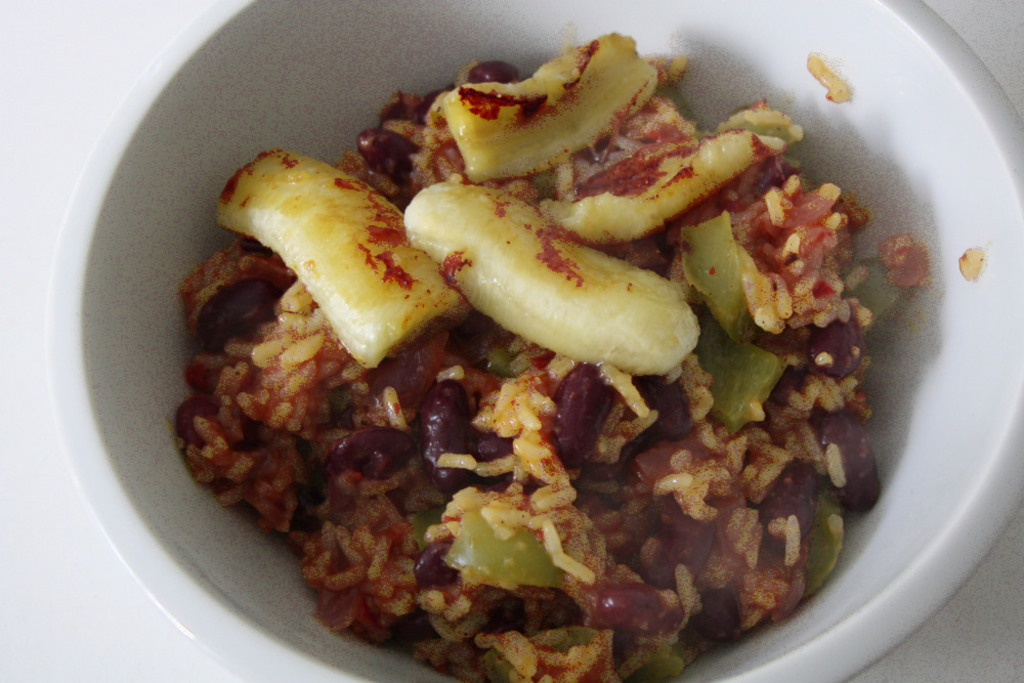
\includegraphics[width=\textwidth]{Kubanisches-Reisgericht/IMG_3600._small.jpg}
\end{center}
\vfill
\mbox{ }
\newpage
